The program is written in Python, using a procedural programming approach.
The program is split across multiple files, for ease of reading.

\section{Data Storage}

The settings data and the config data are stored in two json files, 
\verb|settings.json| and \verb|data.json| respectively.
Listing~\ref*{listing:settings-json} and listing~\ref*{listing:data-json} are
examples of these files, each containing a small amount of data.

\begin{listing}[!ht]
	\inputminted[linenos, fontsize=\footnotesize]{json}{code/settings_template.json}
	\caption{An example of settings.json}
	\label{listing:settings-json}
\end{listing}

\begin{listing}[!ht]
	\inputminted[linenos, fontsize=\footnotesize]{json}{code/data_template.json}
	\caption{An example of data.json}
	\label{listing:data-json}
\end{listing}

In \verb|data.json| object names cannot be changed, but the values can take any 
format, e.g.\ a \verb|teacher|'s \verb|id| could be a string instead.
The same does not apply to \verb|settings.json|, the format of the values must 
stay the same.

\newpage

\section{Debugging}

One bug that I encountered was that the lower and upper bounds of the binary 
search in the \verb|choose_parent| function in \verb|selection.py| were not
updating, as evidenced in figure~\ref*{fig:terminal-output-1}.
\begin{figure}[ht]
	\centering
	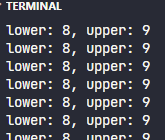
\includegraphics[scale=0.8]{images/binary-search-2}
	\caption{Terminal output showing repeating values of ``lower'' and 
		``upper''}
	\label{fig:terminal-output-1}
\end{figure}

The relevant code is below in figure~\ref*{fig:code-2}
\begin{figure}[ht]
	\centering
	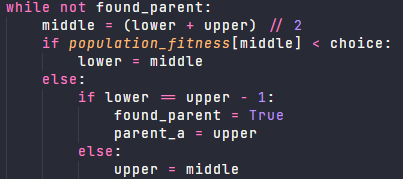
\includegraphics[scale=0.7]{images/binary-search-3}
	\caption{The problem code}
	\label{fig:code-2}
\end{figure}

Changing the order of the \verb|if| \verb|else| statements solved the problem.
\begin{figure}[ht]
	\centering
	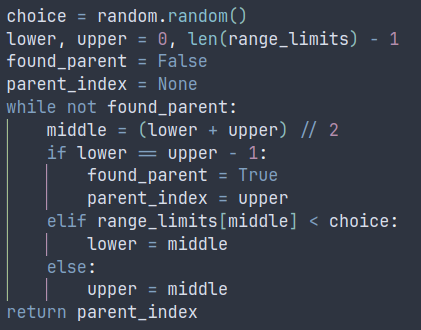
\includegraphics[scale=0.4]{images/binary-search-5}
	\caption{The fixed code}
	\label{fig:code-3}
\end{figure}

\newpage

Another issue I encountered was that after thousands of generations, no valid 
solution was being found, and after further investigation, I discovered that the
population was converging to the same solution.

The first thing I tried doing to fix this was to the increase the chance of a
mutation occurring, as this does help to reduce convergence. 
This was simply done by decreasing the value of \verb|mutation-chance| in 
\verb|settings.json|.
This was not sufficient, and I also found that in several cases, improvements to
the fitness of the overall population (by means of fitter offspring) were 
diminished when they were mutated, as a mutation would often worsen the fitness 
of an individual.
I fixed this by calculating the fitness of the offspring immediately after the 
crossover phase.
If a member of the offspring has fitness that is the same as or worse than the
fitness of the worse parent, then it is mutated, otherwise it is not.
Some pseudocode for this is shown in listing~\ref*{listing:selective-mutation}.

\begin{listing}[!ht]
	\inputminted[linenos, fontsize=\footnotesize]{text}{code/selective-mutation.txt}
	\caption{Only mutating offspring if it does not have improved fitness}
	\label{listing:selective-mutation}
\end{listing}

For this, I also created another function that only returns the fitness values, 
and not a boolean for if there exists a valid solution, and that solution if it
does exist, because they are not needed.
The offspring that are not mutated are added to their own list so that they can
be recombined with the mutated offspring later.
Also note that \verb|SelectParents| also now returns \verb|worstParentFitness| 
so it can be used.

However, this did still not fix the problem of convergence. 
I then decided to change the number of parents involved in the crossover phase,
as it would help to diversify the ``gene pool''.
Additionally, only using two parents to generate very large populations (over 
100 individuals) would counteractive the benefit of the greater population size.
Therefore, it makes more sense for the number of parents to scale with the size
of the population.

So instead of selecting two parents using the previous ``spinner wheel'' method,
the half of the population with the better fitness will be chosen, and four 
offspring will be produced from a pair of parents.

Firstly, I decided to change how the fitness is calculated.
Because I do not need better fitness to be a larger number (as probability is no
longer being used choose the parents), the number of constraint violations is
not inverted, and instead that number is used to denote the fitness, meaning
that now, lower fitness is better, instead of before where higher fitness was 
better.
The pseudocode for this is now shown in listing~\ref*{listing:fitness-new}.

\begin{listing}[!ht]
	\inputminted[linenos, fontsize=\footnotesize]{text}{code/fitness-new.txt}
	\caption{Pseudocode for modified fitness function}
	\label{listing:fitness-new}
\end{listing}

The selection process for the parents is now greatly simplified, as they just
need to be sorted by their fitness, and then the best ones are selected.
However, it is not as simple as selecting half of population, if the size of the
population is an odd number, or if half of the population is an odd number (as 
there be one parent without a partner).
Therefore the size of the population needs to be a multiple of 4.
The pseudocode is now:

\begin{listing}[!ht]
	\inputminted[linenos, fontsize=\footnotesize]{text}{code/selection-new.txt}
	\caption{Pseudocode for modified selection phase}
	\label{listing:selection-new}
\end{listing}

Next, the crossover phase had to be changed so that two parents are chosen
randomly, and they crossover twice, with a random locus each time, to create a 
total of four offspring between the pair of them.

But, I found that if there were multiple parents with the same fitness value,
only one of their chromosomes was being used.
This was due to how the fitness values were stored.
The fitness values were being stored as a list of integers, and the only thing 
that was linking them to which solution they belonged to was the order, as they
were being stored in the same order as the solutions were within the population
list.
This meant that if the index of a fitness value was used to refer to a solution,
the same solution would be referred to multiple times if the same value was in
the fitness value list multiple times. (Note: this is not illustrated in 
previous pseudocode.)

To solve this, I tried to store the fitness values as a dictionary, which stores
data in a list of key:value pairs.
I was going to store each solution as the key, with the corresponding fitness
value as the value.
However, this would not work as the key has to be a string, not a list, which is
the data type each solution is stored as.

Instead, I stored them as a list of pairs, in the format
\begin{Verbatim}[tabsize=4]
[
	[solution1, fitnessValue1],
	[solution2, fitnessValue2],
	...,
	[solutionN, fitnessValueN]
]
\end{Verbatim}
so referencing a fitness value by its index would always return the right 
solution, if needed.

Finally, I noticed that the chromosomes of the chosen parents were changing at
some point between after the selection phase and after the mutation phase.
Through trial and error, I worked out that they were changing when a mutation
occurred. 
This was happening because variables in Python work by pointing at values, 
rather than storing their own copy of a value.
Because of this, when mutating a child's chromosome (which points to the 
parent), the parent's chromosome also mutates.
I fixed this by creating a deep copy (from the \verb|copy| module) of the 
parents, which creates a completely separate variable with an ID which is not
referenced by its offspring, and hence does not change when the offspring does.
Now, my program works as expected.

% #TODO: removing bad ppl